%!TEX root = /Users/stevenmartell/Documents/CONSULTING/HumpbackChub/HBC_2011_Assessment/WRITEUP/HBCmain.tex

\subsection{Sampling effort} % (fold)
\label{sub:sampling_effort}
The database provided for this project contains only records in which humpback chub (HBC) were captured, therefore summary statistics regarding effort for hoop nets and tramel nets are regarded as incomplete because sets that did not capture HBC were not included in these data.

Sampling intensity was greatest in the early 1990s and more recently in the mid to late 2000s, with a peak of 24 trips in 1993 with roughly 174 days fishing on the river (Table \ref{table:Effort}).  The vast majority of humpback chub sampled are captured in hoop nets, and although these data do not include sets with zero catch, trends in the ratio of hoop net catch to hoop net sets has been increasing since about 2005 (Table \ref{table:Effort}).


% latex.default(Effort[-25, ], file = fn, caption = cap, label = "table:Effort",      size = "scriptsize", rowname = NULL) 
%
\begin{table}[!tbp]
 \scriptsize
 \caption{Number of trips,  days fished,  unique sets, 
                  hoop and tramel net sets,  other gears,  catch of humpback
                  chub in hoop nets and tramel nets,  and the corresponding
                  arithmatic CPUE for each gear. Note that these CPUE trends should
                  not be used as a relative abundance index because zero catch of HBC 
                  have been excluded from the effort data.\label{table:Effort}} 
 \begin{center}
 \begin{tabular}{lrrrrrrrrrr}\hline\hline
\multicolumn{1}{c}{Year}&\multicolumn{1}{c}{Trips}&\multicolumn{1}{c}{Days}&\multicolumn{1}{c}{Sets}&\multicolumn{1}{c}{Hoop}&\multicolumn{1}{c}{Tramel}&\multicolumn{1}{c}{Other}&\multicolumn{1}{c}{Hoop Ct}&\multicolumn{1}{c}{Tramel Ct}&\multicolumn{1}{c}{Hoop CPUE}&\multicolumn{1}{c}{Tramel CPUE}\tabularnewline
\hline
1989&$ 2$&$ 29$&$ 256$&$ 182$&$ 82$&$  -8$&$ 560$&$321$&$3.08$&$3.91$\tabularnewline
1990&$ 4$&$ 38$&$ 150$&$  82$&$ 64$&$   4$&$ 473$&$140$&$5.77$&$2.19$\tabularnewline
1991&$14$&$177$&$1370$&$ 976$&$352$&$  42$&$3978$&$711$&$4.08$&$2.02$\tabularnewline
1992&$19$&$172$&$2104$&$1731$&$322$&$  51$&$4740$&$636$&$2.74$&$1.98$\tabularnewline
1993&$24$&$174$&$1941$&$1473$&$374$&$  94$&$6313$&$876$&$4.29$&$2.34$\tabularnewline
1994&$ 8$&$133$&$1032$&$ 962$&$ 70$&$   0$&$2997$&$239$&$3.12$&$3.41$\tabularnewline
1995&$ 7$&$ 84$&$ 543$&$ 511$&$ 32$&$   0$&$2190$&$118$&$4.29$&$3.69$\tabularnewline
1996&$ 2$&$ 34$&$ 105$&$  65$&$ 34$&$   6$&$ 113$&$ 72$&$1.74$&$2.12$\tabularnewline
1997&$ 3$&$ 38$&$  91$&$  48$&$ 41$&$   2$&$  58$&$153$&$1.21$&$3.73$\tabularnewline
1998&$ 8$&$ 51$&$ 188$&$ 165$&$ 17$&$   6$&$ 377$&$ 58$&$2.28$&$3.41$\tabularnewline
1999&$ 9$&$ 47$&$ 201$&$ 169$&$ 19$&$  13$&$ 392$&$ 54$&$2.32$&$2.84$\tabularnewline
2000&$12$&$ 56$&$ 618$&$ 546$&$ 58$&$  14$&$1150$&$ 81$&$2.11$&$1.40$\tabularnewline
2001&$ 7$&$ 58$&$1381$&$1215$&$167$&$  -1$&$4003$&$233$&$3.29$&$1.40$\tabularnewline
2002&$ 9$&$ 61$&$1057$&$1048$&$  6$&$   3$&$3346$&$ 10$&$3.19$&$1.67$\tabularnewline
2003&$15$&$ 94$&$1053$&$ 950$&$ 14$&$  89$&$2058$&$ 27$&$2.17$&$1.93$\tabularnewline
2004&$19$&$115$&$1083$&$ 734$&$ 29$&$ 320$&$1621$&$ 49$&$2.21$&$1.69$\tabularnewline
2005&$17$&$119$&$1323$&$ 914$&$103$&$ 306$&$1919$&$174$&$2.10$&$1.69$\tabularnewline
2006&$19$&$120$&$1221$&$ 995$&$ 31$&$ 195$&$3442$&$ 58$&$3.46$&$1.87$\tabularnewline
2007&$13$&$ 74$&$1413$&$1079$&$144$&$ 190$&$4352$&$225$&$4.03$&$1.56$\tabularnewline
2008&$14$&$208$&$2655$&$1145$&$  0$&$1510$&$4838$&$  0$&$4.23$&$$\tabularnewline
2009&$10$&$235$&$5059$&$1466$&$  0$&$3593$&$7706$&$  0$&$5.26$&$$\tabularnewline
2010&$11$&$ 99$&$2568$&$1266$&$ 31$&$1271$&$5294$&$ 71$&$4.18$&$2.29$\tabularnewline
2011&$ 5$&$218$&$3009$&$1099$&$  0$&$1910$&$5376$&$  0$&$4.89$&$$\tabularnewline
2012&$ 1$&$ 35$&$  89$&$   0$&$  0$&$  89$&$   0$&$  0$&$$&$$\tabularnewline
\hline
\end{tabular}

\end{center}

\end{table}


% subsection sampling_effort (end)


\subsection{Length composition} % (fold)
\label{sub:length_composition}

The length composition of all 81,812 records is summarized in Figure \ref{fig:FIGS_LSMR_fig:CaptureLFbubbles} where the area of each bubble is proportional to the number of fish measured in that length interval.  Note that individual fish may appear more than once in each year as these data summarize the total number of humpback chub captured and measured in a calendar year.  Prior to 1999, individuals less than 150 mm were rarely entered into the database and there are no records of recapturing fish tagged prior to 1999 that were less than 140 mm total length.  Starting sometime in 1999, individuals >100 mm TL and less than 150 mm were being marked as there have been recoveries associated with these individuals (see panels 1999 and later in Figure \ref{fig:FIGS_LSMR_fig:GrowthIncrements}).  In 2001, a large number of fish between the 100-150mm length interval were captured and tagged (Figure \ref{fig:FIGS_LSMR_fig:CaptureLFbubbles}).  Similarly, starting in 2009 a large number of fish in the 100-150mm length interval have been tagged.  Unfortunately, there are no clear modes of numbers-at-length that appear to progress through the size distribution over time; however, these data were obtained from a variety of sampling gears in a variety of locations and do not represent a standardized sampling program that would allow for monitoring of strong/weak cohorts progressing through the size composition data.

\begin{figure}[htbp]
	\centering
		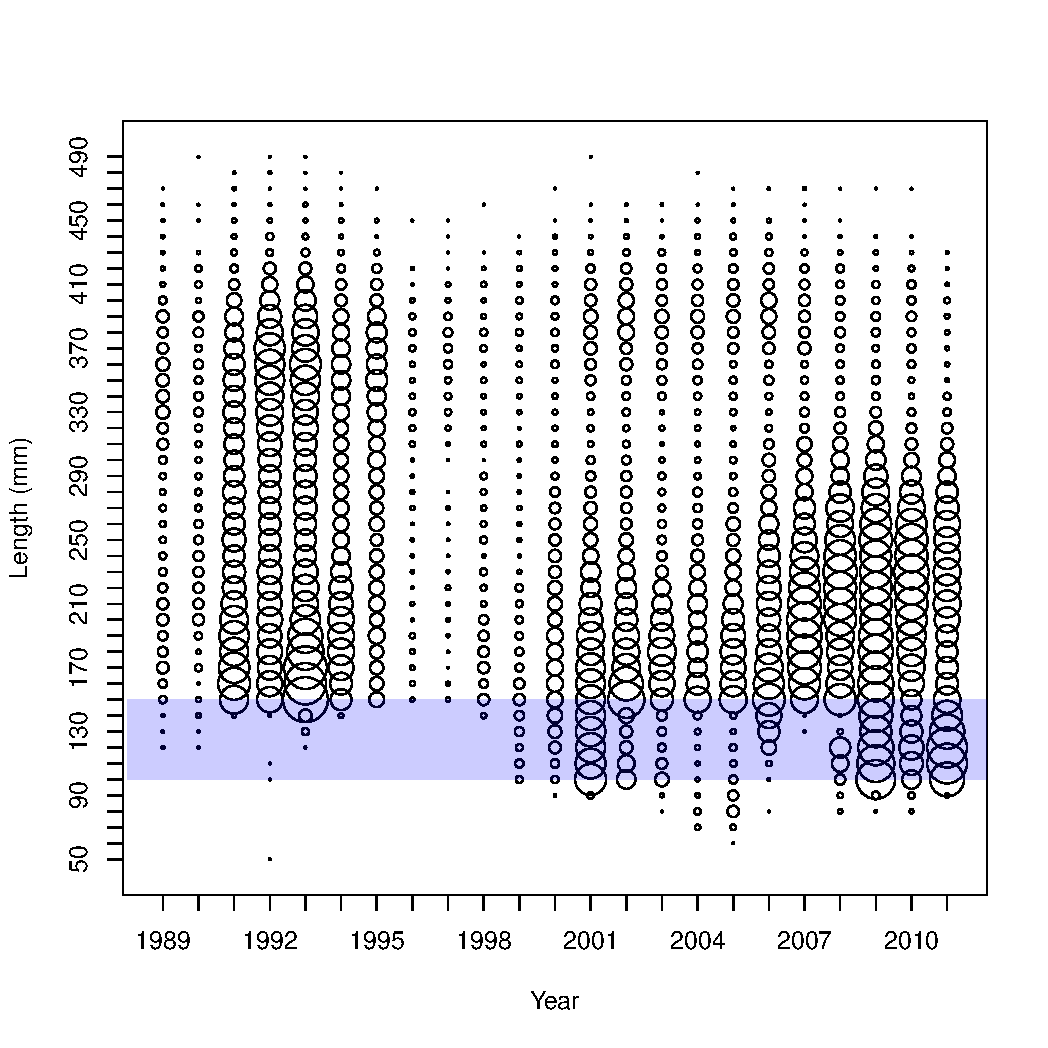
\includegraphics[width=6.5in]{../FIGS/LSMR/fig:CaptureLFbubbles.pdf}
	\caption{Length frequency by year for all gear types. Area of circle is proportional to abundance of measured fish, shaded region represents the 100-150 mm size interval.}
	\label{fig:FIGS_LSMR_fig:CaptureLFbubbles}
\end{figure}

The majority of humpback chub are sampled through the months of April-June and in the fall in September-October (Table \ref{table:Captures}).  Also, the majority of humpback chub are sampled using primarily hoop nets and less so with tramel nets (Table \ref{table:Gear}).  In an attempt to reduce the level of confounding associated with the many different gear types that sample humpback chub, the length composition data was partitioned into two general gear types: (1) hoop nets, ranging in diameter from 2' to 4' with and without bait, and (2) tramel nets of various lengths.  Catch-at-length data by year for hoop nets is shown in Figure \ref{fig:FIGS_LSMR_fig:MarksAtLengthHOOP}.  In the initial years (1989-1990), there are very few recaptures as the marked proportion in the population was relatively low; in subsequent years the marked proportion recaptured increases.  Sampling effort was very low in 1996-1998, resulting in very few fish captured. As time progresses the number of newly marked large fish (greater than 300mm) decreases as most of these individuals were marked in previous years.

\begin{figure}[htbp]
	\centering
		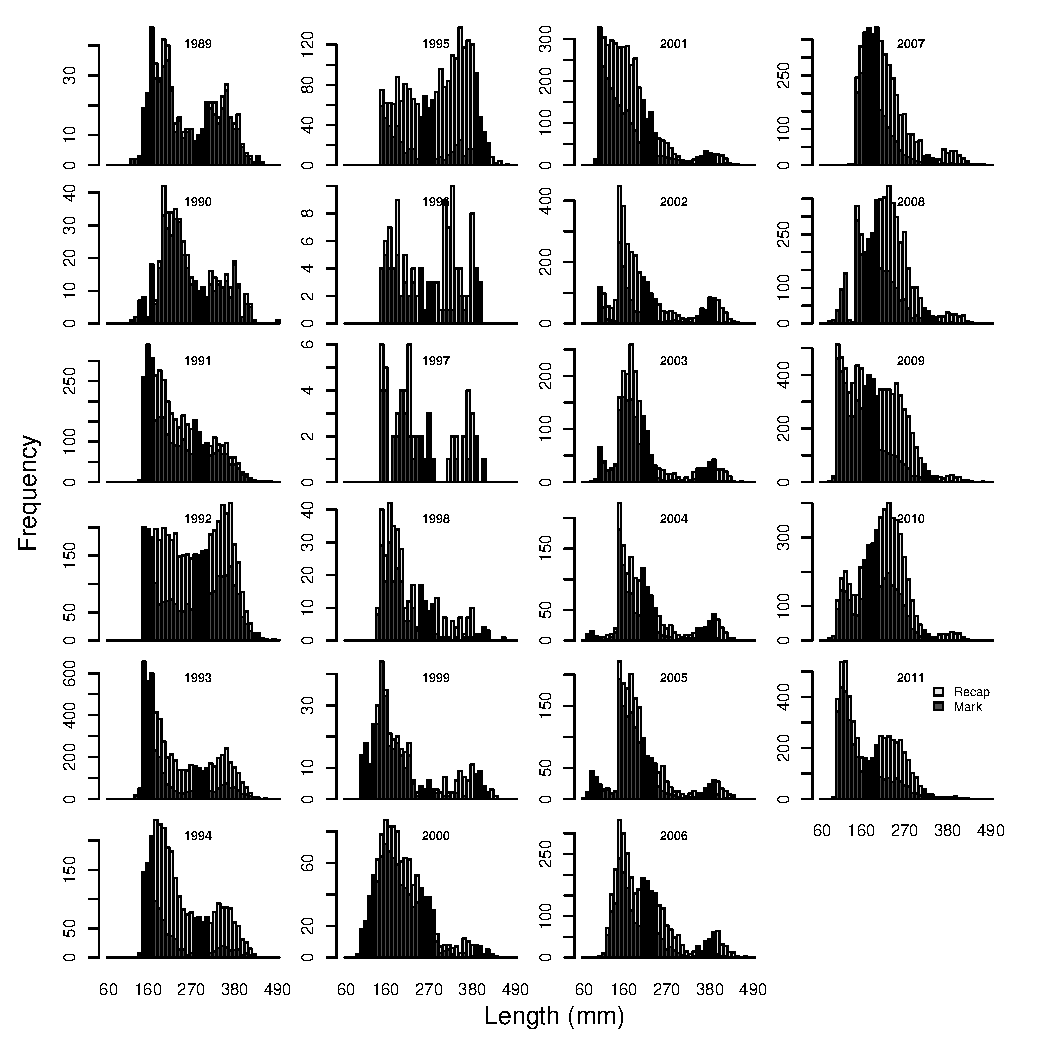
\includegraphics[width=6.5in]{../FIGS/LSMR/fig:MarksAtLengthHOOP.pdf}
	\caption{Annual initial-capture and mark (dark bars) and recapture (light bars) history of HBC using hoop nets (all sizes \& bait) in the LCR and COR reaches from 1989 to 2011.}
	\label{fig:FIGS_LSMR_fig:MarksAtLengthHOOP}
\end{figure}

Far fewer humpback chub have been captured in tramel net gear in comparison to hoopnets, and this is largely due the less frequent use of tramel nets.  Similar patterns in the mark rates were also obtained with the tramel net catch (Figure \ref{fig:FIGS_LSMR_fig:MarksAtLengthGILL}).  Since 1994, tramel net effort for catching humpback chub has been greatly reduced (Table \ref{table:Effort}).  In 2001, the number of tramel net sets with non-zero catches of humpback chub increased to 167 sets, with a very large recapture proportion for fish greater than 300mm.  This observation is also consistent with the large recapture proportion of $>$300mm fish in the hoop net sets in 2001.  Similarly, in 2007, 225 humpback chub were caught in 144 non-zero tramel net sets and the majority of these fish were less than 250mm and never previously marked (Figure \ref{fig:FIGS_LSMR_fig:MarksAtLengthGILL}). Again, this is also consistent with the large number of unmarked fish less than 250mm captured in hoop nets in 2007.

\begin{figure}[htbp]
	\centering
		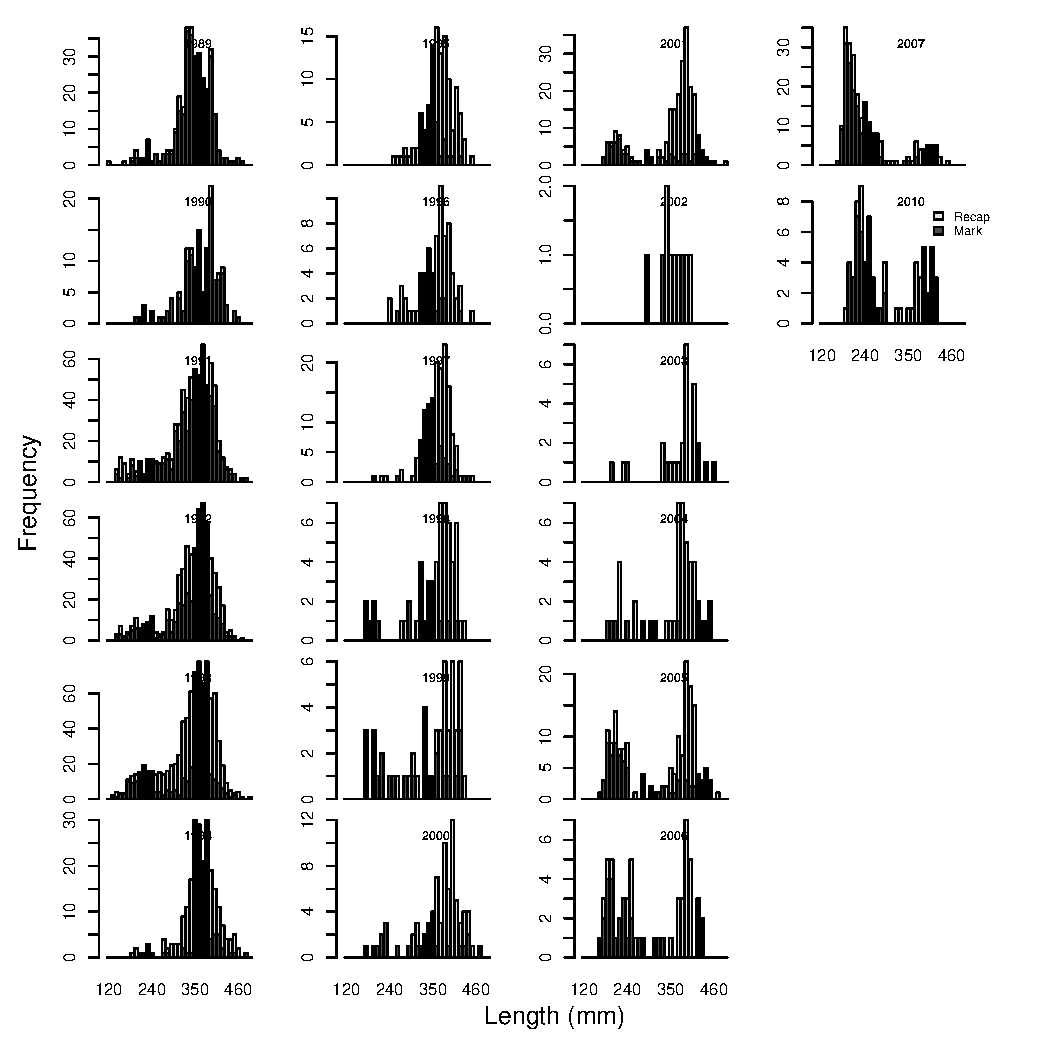
\includegraphics[width=6.5in]{../FIGS/LSMR/fig:MarksAtLengthGILL.pdf}
	\caption{Annual capture and recapture history of HBC using tramel nets of all sizes in the LCR and COR reaches from 1989 to 2011.}
	\label{fig:FIGS_LSMR_fig:MarksAtLengthGILL}
\end{figure}

% latex.default(tx, file = fn, rowname = NULL, caption = cap, size = "footnotesize",      cgroup = cgrp, n.cgroup = ncgrp, label = "table:Captures") 
%
\begin{table}[!tbp]
 \footnotesize
 \caption{Number of fish measured by year and month, sampled by all gears
                  in all reaches of both the LRC and COR.\label{table:Captures}} 
 \begin{center}
 \begin{tabular}{lcrrrrrrrrrrrrr}\hline\hline
\multicolumn{1}{c}{\bfseries }&
\multicolumn{1}{c}{\bfseries }&
\multicolumn{13}{c}{\bfseries MONTH}
\tabularnewline \cline{1-15}
\multicolumn{1}{c}{YEAR}&\multicolumn{1}{c}{}&\multicolumn{1}{c}{1}&\multicolumn{1}{c}{2}&\multicolumn{1}{c}{3}&\multicolumn{1}{c}{4}&\multicolumn{1}{c}{5}&\multicolumn{1}{c}{6}&\multicolumn{1}{c}{7}&\multicolumn{1}{c}{8}&\multicolumn{1}{c}{9}&\multicolumn{1}{c}{10}&\multicolumn{1}{c}{11}&\multicolumn{1}{c}{12}&\multicolumn{1}{c}{(all)}\tabularnewline
\hline
1989&&$  0$&$   0$&$   0$&$    0$&$  887$&$    0$&$   0$&$   0$&$   0$&$   0$&$   0$&$  0$&$  887$\tabularnewline
1990&&$  0$&$   0$&$   0$&$  408$&$  125$&$    0$&$   0$&$   0$&$   0$&$  43$&$  42$&$  0$&$  618$\tabularnewline
1991&&$ 79$&$   3$&$ 135$&$    9$&$  285$&$  394$&$1624$&$1054$&$ 536$&$ 291$&$ 200$&$176$&$ 4786$\tabularnewline
1992&&$168$&$ 340$&$ 781$&$ 1293$&$  493$&$ 1181$&$ 369$&$ 145$&$ 144$&$ 290$&$ 267$&$  0$&$ 5471$\tabularnewline
1993&&$117$&$ 153$&$1132$&$  759$&$ 1359$&$  822$&$ 953$&$1093$&$ 270$&$ 228$&$ 250$&$239$&$ 7375$\tabularnewline
1994&&$154$&$ 201$&$ 296$&$  658$&$  707$&$  410$&$ 198$&$ 154$&$ 152$&$ 129$&$ 128$&$ 55$&$ 3242$\tabularnewline
1995&&$226$&$ 231$&$ 383$&$  915$&$  476$&$   83$&$   0$&$   0$&$   2$&$   0$&$   0$&$  0$&$ 2316$\tabularnewline
1996&&$  0$&$   2$&$  20$&$   96$&$   47$&$    6$&$   0$&$   0$&$  27$&$   0$&$   0$&$  0$&$  198$\tabularnewline
1997&&$  0$&$   0$&$   7$&$   42$&$  114$&$   18$&$   0$&$   0$&$  32$&$   0$&$   0$&$  0$&$  213$\tabularnewline
1998&&$  0$&$   0$&$   1$&$  234$&$   47$&$   36$&$  39$&$  65$&$   5$&$  18$&$   0$&$  0$&$  445$\tabularnewline
1999&&$ 20$&$   0$&$   0$&$  210$&$   52$&$   18$&$   0$&$   0$&$  62$&$  56$&$  53$&$  0$&$  471$\tabularnewline
2000&&$ 20$&$   0$&$   0$&$  418$&$   21$&$  271$&$   2$&$  44$&$  20$&$ 333$&$ 151$&$ 13$&$ 1293$\tabularnewline
2001&&$  0$&$   0$&$   1$&$   37$&$  491$&$ 1347$&$   9$&$ 163$&$  85$&$1180$&$ 929$&$  0$&$ 4242$\tabularnewline
2002&&$  0$&$   4$&$   0$&$  980$&$ 1066$&$    0$&$  20$&$   0$&$ 789$&$ 502$&$   0$&$  0$&$ 3361$\tabularnewline
2003&&$ 16$&$  16$&$  48$&$  599$&$  434$&$    0$&$  55$&$  13$&$ 293$&$ 694$&$  21$&$  0$&$ 2189$\tabularnewline
2004&&$ 18$&$  25$&$  51$&$  760$&$  353$&$   23$&$  27$&$  15$&$ 166$&$ 542$&$  32$&$  0$&$ 2012$\tabularnewline
2005&&$ 23$&$  12$&$  44$&$  515$&$  207$&$  285$&$  93$&$  19$&$ 799$&$ 476$&$   0$&$  0$&$ 2473$\tabularnewline
2006&&$ 24$&$  35$&$ 160$&$ 1098$&$  921$&$  679$&$ 179$&$  56$&$ 270$&$ 317$&$   0$&$  0$&$ 3739$\tabularnewline
2007&&$  0$&$   0$&$   2$&$  937$&$ 1545$&$  900$&$  10$&$   0$&$ 805$&$ 569$&$   0$&$  0$&$ 4768$\tabularnewline
2008&&$  0$&$   5$&$   3$&$ 1265$&$ 1735$&$  528$&$1020$&$ 195$&$ 718$&$ 928$&$   0$&$  0$&$ 6397$\tabularnewline
2009&&$  0$&$   0$&$   6$&$ 1225$&$ 4180$&$ 2267$&$ 551$&$ 168$&$ 895$&$1323$&$ 443$&$245$&$11303$\tabularnewline
2010&&$  0$&$   0$&$   2$&$    0$&$ 1466$&$ 2882$&$ 523$&$  14$&$1043$&$ 708$&$   0$&$  0$&$ 6638$\tabularnewline
2011&&$  0$&$   0$&$   0$&$    0$&$ 2796$&$ 2537$&$ 127$&$ 128$&$ 544$&$1042$&$  63$&$ 49$&$ 7286$\tabularnewline
2012&&$ 28$&$  61$&$   0$&$    0$&$    0$&$    0$&$   0$&$   0$&$   0$&$   0$&$   0$&$  0$&$   89$\tabularnewline
(all)&&$893$&$1088$&$3072$&$12458$&$19807$&$14687$&$5799$&$3326$&$7657$&$9669$&$2579$&$777$&$81812$\tabularnewline
\hline
\end{tabular}

\end{center}

\end{table}


% latex.default(tx, file = fn, rowname = NULL, caption = cap, size = "footnotesize",      cgroup = cgrp, n.cgroup = ncgrp, label = "table:Gear") 
%
\begin{table}[!tbp]
 \footnotesize
 \caption{Number of fish captured by gear type listed in the GCMRC database
                  for each year.\label{table:Gear}} 
 \begin{center}
 \begin{tabular}{lcrrrrrrrrrr}\hline\hline
\multicolumn{1}{c}{\bfseries }&
\multicolumn{1}{c}{\bfseries }&
\multicolumn{10}{c}{\bfseries YEAR}
\tabularnewline \cline{1-12}
\multicolumn{1}{c}{YEAR}&\multicolumn{1}{c}{}&\multicolumn{1}{c}{ANGL}&\multicolumn{1}{c}{DIP}&\multicolumn{1}{c}{ELEC}&\multicolumn{1}{c}{GILL}&\multicolumn{1}{c}{HOOP}&\multicolumn{1}{c}{PA}&\multicolumn{1}{c}{SEINE}&\multicolumn{1}{c}{TRAP}&\multicolumn{1}{c}{(all)}&\multicolumn{1}{c}{NA}\tabularnewline
\hline
1989&&$ 6$&$0$&$  0$&$ 321$&$  560$&$   0$&$  0$&$ 0$&$  887$&$ 0$\tabularnewline
1990&&$ 2$&$0$&$  3$&$ 140$&$  473$&$   0$&$  0$&$ 0$&$  618$&$ 0$\tabularnewline
1991&&$ 4$&$0$&$ 44$&$ 711$&$ 3978$&$   0$&$ 11$&$ 1$&$ 4786$&$37$\tabularnewline
1992&&$ 3$&$0$&$ 68$&$ 636$&$ 4740$&$   0$&$ 24$&$ 0$&$ 5471$&$ 0$\tabularnewline
1993&&$ 2$&$0$&$ 80$&$ 876$&$ 6313$&$   0$&$102$&$ 1$&$ 7375$&$ 1$\tabularnewline
1994&&$ 1$&$0$&$  1$&$ 239$&$ 2997$&$   0$&$  2$&$ 1$&$ 3242$&$ 1$\tabularnewline
1995&&$ 1$&$0$&$  7$&$ 118$&$ 2190$&$   0$&$  0$&$ 0$&$ 2316$&$ 0$\tabularnewline
1996&&$ 0$&$0$&$  4$&$  72$&$  113$&$   0$&$  9$&$ 0$&$  198$&$ 0$\tabularnewline
1997&&$ 0$&$0$&$  2$&$ 153$&$   58$&$   0$&$  0$&$ 0$&$  213$&$ 0$\tabularnewline
1998&&$ 0$&$0$&$  5$&$  58$&$  377$&$   0$&$  4$&$ 1$&$  445$&$ 0$\tabularnewline
1999&&$ 0$&$0$&$ 17$&$  54$&$  392$&$   0$&$  1$&$ 7$&$  471$&$ 0$\tabularnewline
2000&&$ 0$&$0$&$  6$&$  81$&$ 1150$&$   0$&$ 55$&$ 1$&$ 1293$&$ 0$\tabularnewline
2001&&$ 5$&$0$&$  1$&$ 233$&$ 4003$&$   0$&$  0$&$ 0$&$ 4242$&$ 0$\tabularnewline
2002&&$ 0$&$0$&$  5$&$  10$&$ 3346$&$   0$&$  0$&$ 0$&$ 3361$&$ 0$\tabularnewline
2003&&$ 0$&$1$&$102$&$  27$&$ 2058$&$   0$&$  1$&$ 0$&$ 2189$&$ 0$\tabularnewline
2004&&$ 2$&$0$&$108$&$  49$&$ 1621$&$ 226$&$  0$&$ 0$&$ 2012$&$ 6$\tabularnewline
2005&&$ 0$&$0$&$228$&$ 174$&$ 1919$&$ 152$&$  0$&$ 0$&$ 2473$&$ 0$\tabularnewline
2006&&$ 0$&$0$&$138$&$  58$&$ 3442$&$ 100$&$  1$&$ 0$&$ 3739$&$ 0$\tabularnewline
2007&&$ 0$&$0$&$  9$&$ 225$&$ 4352$&$ 181$&$  1$&$ 0$&$ 4768$&$ 0$\tabularnewline
2008&&$ 3$&$0$&$  8$&$   0$&$ 4838$&$1527$&$ 21$&$ 0$&$ 6397$&$ 0$\tabularnewline
2009&&$ 0$&$0$&$  6$&$   0$&$ 7706$&$3589$&$  0$&$ 2$&$11303$&$ 0$\tabularnewline
2010&&$ 3$&$0$&$  0$&$  71$&$ 5294$&$1269$&$  0$&$ 0$&$ 6638$&$ 1$\tabularnewline
2011&&$ 0$&$0$&$  0$&$   0$&$ 5376$&$1910$&$  0$&$ 0$&$ 7286$&$ 0$\tabularnewline
2012&&$ 0$&$0$&$  0$&$   0$&$    0$&$  89$&$  0$&$ 0$&$   89$&$ 0$\tabularnewline
(all)&&$32$&$1$&$842$&$4306$&$67296$&$9043$&$232$&$14$&$81812$&$46$\tabularnewline
\hline
\end{tabular}

\end{center}

\end{table}


% subsection length_composition (end)

